%%%%%%%%%%%%%%%%%%%%%%%%%%%%%%%%%%%%%%%%%%%%%%%%%%%%%%%%%%%%%%%%%%%
%%% Documento LaTeX 											%%%
%%%%%%%%%%%%%%%%%%%%%%%%%%%%%%%%%%%%%%%%%%%%%%%%%%%%%%%%%%%%%%%%%%%
% Título:	Plantilla de TFG/TFM
% Autor:  Ignacio Moreno Doblas
% Fecha:  2014-02-01, actualizado 2019-11-11
%%%%%%%%%%%%%%%%%%%%%%%%%%%%%%%%%%%%%%%%%%%%%%%%%%%%%%%%%%%%%%%%%%%
%	Modo:					PDFLaTeX.
%%%%%%%%%%%%%%%%%%%%%%%%%%%%%%%%%%%%%%%%%%%%%%%%%%%%%%%%%%%%%%%%%%%

% Preámbulo del documento.
%-----------------------------------------------------------------%
% Clase de documento: libro
\documentclass[12pt,a4paper]{book} % article, report, book.

% Preámbulo: paquetes, comandos, entornos, estilos y título de página.
%%%%%%%%%%%%%%%%%%%%%%%%%%%%%%%%%%%%%%%%%%%%%%%%%%%%%%%%%%%%%%%%%%%
%%% Documento LaTeX 																						%%%
%%%%%%%%%%%%%%%%%%%%%%%%%%%%%%%%%%%%%%%%%%%%%%%%%%%%%%%%%%%%%%%%%%%
% Título:	Paquetes
% Autor:  Ignacio Moreno Doblas
% Fecha:  2014-02-01, actualizado 2019-11-11
%%%%%%%%%%%%%%%%%%%%%%%%%%%%%%%%%%%%%%%%%%%%%%%%%%%%%%%%%%%%%%%%%%%
% Tabla de materias:
%	1 Codificación e idioma %
% 2 Matemáticas y Física %
% 3 Gráficos%
% 4 Estilo y formato%
%%%%%%%%%%%%%%%%%%%%%%%%%%%%%%%%%%%%%%%%%%%%%%%%%%%%%%%%%%%%%%%%%%%

%1 Codificación e idioma%
\usepackage[utf8]{inputenc} %Codificación en latin-1%
\usepackage[T1]{fontenc} %Codificación de fuente%
\usepackage[spanish]{babel}	%Hyphenation (Guionado) en español%
\usepackage{eurosym} %Tipografía euro (€)%

%2 Matemáticas y Física %
% Importante para ecuaciones, magnitudes y unidades%
\usepackage{amssymb,amsmath,latexsym,amsfonts} % paquetes estándar%
\usepackage[squaren]{SIunits} %Paquete para magnitudes y unidades físicas%
\usepackage{ifthen} %sentencias if y while%

%3 Gráficos%
\usepackage{graphics,graphicx,subcaption} %paquetes gráficos estándar%
%\usepackage{subfigure} %permite varias subfiguras en una figura
\usepackage{wrapfig} %paquete para gráfica lateral%
\usepackage{float} %figuras flotantes%
	% \begin{floatingfigure}[r]/[l]{4.5cm}
	% \end{floatingfigure}
\usepackage{graphpap}	%comando \graphpaper en el entorno picture%

%4 Estilo y formato%
\usepackage{imakeidx} %MakeIndex%
%Comando para crear glosario (index en inglés)
\makeindex[columns=2, title=Glosario, intoc]
%\usepackage{showidx} % Hace que cada comando \index se imprima en la página donde se ha puesto (útil para corregir los índices)
\usepackage{fancyhdr}	%cabeceras y pies mejor que con \pagestyle{}%
\setlength{\headheight}{16pt}% ...at least 16pt
\usepackage{titlesec,titletoc} %Formateo de secciones y títulos%
\raggedbottom %Para fragmentar versos en varias páginas%
\usepackage{alltt} % Define el environment alltt, como verbatim, excepto que \, { y } tienen su significado normal. Se describe en el fichero alltt.dtx.
\usepackage[pdftex,bookmarksnumbered,hidelinks]{hyperref} %hyper-references%
\usepackage{minitoc} % Para poner tablas de contenido en cada capítulo.
\usepackage{listings} % Para escribir piezas de código C, Python, etc. %
%listings configuration
\lstset{
  language=Python, %Puede ser C, C++, Java, etc.
  showstringspaces=false,
  formfeed=\newpage,
  tabsize=4,
  commentstyle=\itshape,
  basicstyle=\footnotesize\ttfamily,
  escapeinside={(@}{@)},
  morekeywords={models, lambda, forms}
}
\renewcommand{\lstlistingname}{Listado}

\usepackage{tipa} % tipografía IPA (International Phonetic Alphabet)
\usepackage{longtable} %Entorno Longtable, fracciona tablas a lo largo de páginas%
\usepackage{xcolor}
\usepackage{colortbl}
\usepackage{acronym}  %Para expandir automáticamente los acrónimos
\usepackage{emptypage} %Para eliminar el número de página en páginas sin contenido (\cleardoublepage)

\usepackage{tikz}


%%%%%%%%%%%%%%%%%%%%%%%%%%%%%%%%%%%%%%%%%%%%%%%%%%%%%%%%%%%%%%%%%%%
%%% Documento LaTeX 											%%%
%%%%%%%%%%%%%%%%%%%%%%%%%%%%%%%%%%%%%%%%%%%%%%%%%%%%%%%%%%%%%%%%%%%
% Título:	Comandos
% Autor:  Ignacio Moreno Doblas
% Fecha:  2014-02-01, actualizado 2019-11-11
%%%%%%%%%%%%%%%%%%%%%%%%%%%%%%%%%%%%%%%%%%%%%%%%%%%%%%%%%%%%%%%%%%%
% Tabla de materias:
% 1 Información del Documento %
% 2 Comandos a nivel de texto %
% 3 Comandos a nivel de entorno %
% 4 Comandos a nivel de página y sección %
% 5 Otros comandos %
%%%%%%%%%%%%%%%%%%%%%%%%%%%%%%%%%%%%%%%%%%%%%%%%%%%%%%%%%%%%%%%%%%%

% 1 Información del Documento %
\newcommand{\tfgtitlename}{<Título del Trabajo Fin de Grado>}
\newcommand{\tfgtitlenameENG}{<Título del TFG en inglés>}
\newcommand{\tfgauthorname}{<Nombre del autor>}
\newcommand{\tfgtutorname}{<Nombre del tutor>}
\newcommand{\tfganno}{<año de publicación>}

% 2 Comandos a nivel de texto %
\newcommand{\R}{\textsuperscript{\textregistered}}	%Símbolo registrado%
\newcommand{\C}{\textsuperscript{\copyright}}	%Símbolo Copyright%
\newcommand{\TM}{\texttrademark} %Símbolo Trade Mark (marca comercial)%

% 2.1 Comandos abreviatura %
\newcommand{\tit}{\textit} %Fuente cursiva (itálica)%
\newcommand{\tbf}{\textbf} %Fuente negrita%
\newcommand{\ttw}[1]{\texttt{#1}} %Fuente máquina de escribir (typewriter)%
%Combinación%
\newcommand{\textittt}[1]{\textit{\texttt{#1}}} %itálica y typewriter%
\newcommand{\textittw}{\textittt} % Otra forma de escribirlo.
\newcommand{\tittw}{\textittw} %Shortened%
\newcommand{\tbftw}[1]{\tbf{\ttw{#1}}}

%Crea una nueva línea y la indenta sin crear interlineado extra.
\newcommand{\nli}{\\ \indent}

%Para escribir un correo electrónico%
\newcommand{\mailto}[1]{\href{mailto:#1}{#1}}

% Si vas a hacer un uso básico de \index (entradas en el índice de sólo un nivel, sin formatos especiales, etc.), define la orden
\newcommand{\miindex}[1]{#1\index{#1}}

\newcommand{\hs}{\hspace} % Abreviatura espacio horizontal
\newcommand{\vs}{\vspace} % Abreviatura espacio vertical

% Abreviaturas para los conjuntos de números más comunes.
\newcommand{\realnumbers}{\mathbb R}
\newcommand{\naturalnumbers}{\mathbb N}
\newcommand{\integernumbers}{\mathbb Z}
\newcommand{\rationalnumbers}{\mathbb Q}
\newcommand{\complexnumbers}{\mathbb R}
\newcommand{\irrationalnumbers}{\mathbb I}

% Doble barra sobre una letra (para expresar las matrices).
\newcommand{\doublebar}[1]{\bar{\bar{#1}}}
% Ej: \vector(y) = \doublebar(A) \vector(x) (Stma. lineal de ec.)

% 3 Comandos a nivel de entorno %
\newcommand{\benu}{\begin{enu}} % Begin enumerate
\newcommand{\eenu}{\end{enu}} 	% End enumeration

%Comando para escribir código Python
\newcommand{\code}[3]{
\begin{minipage}{0.96\linewidth}
\begin{center}
    \lstinputlisting[
        language   = Python,
        frame      = lines,
        framexleftmargin = 5mm,
        caption    = {#1},
        label      = {#3},
    ]{#2}
\end{center}
\end{minipage}
}

% 4 Comandos a nivel de página y sección %
%Crea página en blanco
\newcommand{\blankpage}{\clearpage{\pagestyle{empty}\cleardoublepage}}

% Versión x del comando section: sin numeración pero sí aparece en la tabla de contenidos.
\newcommand{\sectionx}[1]{
	\section*{#1}
	\addcontentsline{toc}{section}{#1}
}

% Versión y del comando section: sin numeración y NO aparece en la tabla de contenidos.
\newcommand{\sectiony}[1]{
	\section*{#1}
}

% Versión x del comando chapter: sin numeración pero sí  aparece en la tabla de contenidos.
\newcommand{\chapterx}[1]{
	\chapter*{#1}
	%\addcontentsline{toc}{chapter}{#1} %Caused by minitoc package%
	\addstarredchapter{#1} %For minitoc package%
}

% substituto del comando \chapter: incluye estilo de página.
\newcommand{\chapterbegin}[1]%
	{%
		\pagestyle{fancy}
		\renewcommand{\headrulewidth}{1pt}
		\fancyhead[LE,RO]{\thepage}
		\fancyhead[RE]{Capítulo \thechapter. #1}
		%\fancyhead[RE]{Parte \thepart \rightmark} %
		\fancyhead[LO]{\nouppercase{\rightmark}} %
		\fancyfoot[CE,CO]{} %

		\chapter{#1}
	}

% Versión x del comando \chapterbegin: sin numeración y aparece en la tabla de contenidos.
\newcommand{\chapterbeginx}[1]%
	{%
		\pagestyle{fancy}
		\renewcommand{\headrulewidth}{1pt}
		\fancyhead[RO,LE]{\thepage}
		\fancyhead[RE,LO]{#1}
		%\fancyhead[LO]{Chapter \thechapter}
		%\fancyhead[RE]{Part \thepart} %
		\fancyfoot[CE,CO]{} %
		
		\chapterx{#1}
	}

%Fin de capítulo
\newcommand{\chapterend}{
\cleardoublepage 
\thispagestyle{empty}
}
%Si fuera un artículo en lugar un libro, \clearpage en lugar de \cleardoublepage

% 5 Otros comandos %
%\let\Oldpart\part
%\newcommand{\parttitle}{}
%\renewcommand{part}[1]{\Oldpart{#1}\renewcommand{\parttitle}{#1}} %Header customization%

%Cambiar el título índice de capítulo a ``Contenido''.
\renewcommand{\mtctitle}{Contenido}

\dominitoc % Para tablas de contenidos por capítulo.

\addto{\captionsspanish}{
	\renewcommand{\listtablename}{Índice de Tablas}
	\renewcommand{\tablename}{Tabla} } % Por ejemplo, modificar el nombre de 'Cuadro' a 'Tabla'.

\addto{\captionsspanish}{
	\renewcommand{\contentsname}{Índice} }

% Si se desea cambiar el tipo de letra a Computer Modern
% por cualquier razón, comenta las siguientes
% dos líneas
\renewcommand{\rmdefault}{phv} % Arial
\renewcommand{\sfdefault}{phv} % Arial

%\addto{\captionsspanish}{
%	\renewcommand{\partname}{Fase} }

%\addto{\captionsspanish}{%
%    \renewcommand{\refname}{\vspace{-4.5ex}}} % Para que no aparezca el texto 'referencias' en la bibliografía.

% Modifica el interlineado
%\renewcommand{\baselinestretch}{1.5}

%%%%%%%%%%%%%%%%%%%%%%%%%%%%%%%%%%%%%%%%%%%%%%%%%%%%%%%%%%%%%%%%%%%
%%% Documento LaTeX 																						%%%
%%%%%%%%%%%%%%%%%%%%%%%%%%%%%%%%%%%%%%%%%%%%%%%%%%%%%%%%%%%%%%%%%%%
% Título:	Entornos
% Autor:  Ignacio Moreno Doblas
% Fecha:  2014-02-01, actualizado 2019-11-11
%%%%%%%%%%%%%%%%%%%%%%%%%%%%%%%%%%%%%%%%%%%%%%%%%%%%%%%%%%%%%%%%%%%
% Tabla de materias:
%--------------------%
% 1 dobleindent
% 2 izqindent
% 3 dobleindentx
% 4 ite
% 5 descript
% 6 enu
% 7 itemization
% 8 sinopsis
%%%%%%%%%%%%%%%%%%%%%%%
% Para conocer los parámetros de diseño de las listas, tales como
%  los márgenes izquierdo, derechos y los diferentes saltos,
%  véase el archivo ``List layout.png'' que acompaña esta plantilla.
% Así se conocerá mejor cómo adaptar un entorno según los requisitos
%  del usuario.

%%%%%%%%%%%%%%%%%%%%%%%
% Definición de longitudes para usar en los entornos:
%
% Normal parskip.
\newlength{\parskipenv}
\setlength{\parskipenv}{\parskip}

\newlength{\parindentenv}
\setlength{\parindentenv}{\parindent}
%%%%%%%%%%%%%%%%%%%%%%%

% 1 dobleindent
%El entorno dobleindent está pensando para escribir párrafos con doble indentación a cada lado.
%Tiene dos parámetros de entrada con las distancias medidas desde los márgenes de página.

\newenvironment{dobleindent}[2]
	%Comienzo de nuevo entorno%
	{
	\begin{list}
		{}
		{
		% Left and right margins:
		\leftmargin = #1
		\rightmargin = #2
		%
		% Separation from preceding and following text:
		\topsep = 0ex
		\partopsep = 0ex
		\parsep = \parskipenv
		%
		% Indentation for paragraphs:
		\itemsep = \parskipenv
		\itemindent = \parindentenv
		\listparindent = \itemindent
		%
		% Horizontal separation from label:
		\labelsep = 1ex
		\settowidth{\labelwidth}{0cm}
		}

		 \item}
	% End new env
	{\end{list}}

%%%%%%%%%%%%%%%%%%%%%%%%%%%%%
%2 izqindent
% El entorno izqindent sólo crea un párrafo indentado a la izquierda.
\newenvironment{izqindent}[1]
{
\begin{dobleindent}{#1}{0cm}
}
{
\end{dobleindent}
}

%%%%%%%%%%%%%%%%%%%%%%%%%%%%%
% 3 dobleindentx
% El entorno dobleindentx es una variación del dobleindent usando leftskip y rightskip.
% Aunque es más limitado, también se puede usar.
\newenvironment{dobleindentx}[2] % Sólo funciona en modo paragraph
{ % Preamble
  \leftskip = #1
  \rightskip = #2
}
{ % Postamble
\leftskip = 0cm
\rightskip = 0cm
}

%%%%%%%%%%%%%%%%%%%%%%%%%%%%%
% 4 ite
% El entorno ite es una modificación del entorno itemize estándar de \LaTeX. Puede usarse o modificarse si el usuario lo desea.
% También puede parametrizarse el entorno enumerate o description de forma equivalente.
\newenvironment{ite}
	{
		\begin{izqindent}{\parindent}
		\hspace{-\parindent} 	% compensación del sangrado que introduce el entorno.
		\vspace{-1.0\parskip}	% compensación del \parskip que introduce el entorno.
		\vspace{-\baselineskip}	% compensación por la línea que introduce el entorno.
		\begin{itemize}
	}
	{
		\end{itemize}
		\end{izqindent}
	}

%%%%%%%%%%%%%%%%%%%%%5
% commando stdformat para formatear los entornos descript, enu y itemization.
\newcommand{\stdformat}
	{% Declarations for format presentation.
		%
		% Separation from preceding and following text:
		\setlength{\topsep}{1ex}%
		\setlength{\partopsep}{0ex} %
		%
		% Horizontal separation from label:
		\labelsep = 1ex
		\setlength{\labelwidth}{0ex}
		%
		%	Left and right margins:
		\setlength{\leftmargin}{1cm}%
		\addtolength{\leftmargin}{\labelsep}
		\setlength{\rightmargin}{0ex}
		%
		% Indentation for paragraphs:
		\setlength{\itemindent}{-\leftmargin}%
		\addtolength{\itemindent}{1ex}
		\setlength{\listparindent}{\parindent}%
		%
		% Separation between paragraphs.
		\setlength{\parsep}{\parskipenv}%
		\setlength{\itemsep}{1ex}
	}

%%%%%%%%%%%%%%%%%%%%%%%%%%%%%
% 5 descript

\newenvironment{descript}
	% Beginning new env def.
	{
		\begin{list}
			{} % No default label for \item.
			{
				% Declarations for format presentation.
				\stdformat
				%
				\renewcommand{\makelabel}[1]{\normalfont\bfseries##1\hfil}
			}
	}
	% Ending new env def.
	{
		\hspace*{\fill} \\ \end{list}
	} % Se introduce un salto de línea para que el texto siguiente esté separado.
%END newenvironment{descript}

%%%%%%%%%%%%%%%%%%%%%%%%%%%%%
% 6 enu
\newcounter{itemnumber} % Counter for the environment.

\newenvironment{enu}
	% Beginning new env def.
	{
		\begin{list}
		{
			\raggedleft \arabic{itemnumber}
		}
		{
			\usecounter{itemnumber}
			\stdformat
		}
	}
	{
		\end{list}
	}

%%%%%%%%%%%%%%%%%%%%%%%%%%%%%
% 7 itemization
\newenvironment{itemization}
	% Beginning new env def.
	{
		\begin{list}
			{$\bullet$} % No default label for \item.
			{
				% Declarations for format presentation.
				\stdformat
			}
	}
	% Ending new env def.
	{
		\end{list}
	}


%%%%%%%%%%%%%%%%%%%%%%%%%%%%%
% 8 sinopsis
\newenvironment{sinopsis}{%[1]{
	\sectiony{Sinopsis}
	%\label{#1}
} {
%	\pagebreak
}

%%%%%%%%%%%%%%%%%%%%%%%%%%%%%%%%%%%%%%%%%%%%%%%%%%%%%%%%%%%%%%%%%%%
%%% Documento LaTeX 																						%%%
%%%%%%%%%%%%%%%%%%%%%%%%%%%%%%%%%%%%%%%%%%%%%%%%%%%%%%%%%%%%%%%%%%%
% Título:	Parámetros de estilo
% Autor:  Ignacio Moreno Doblas
% Fecha:  2014-02-01, actualizado 2019-11-11
%%%%%%%%%%%%%%%%%%%%%%%%%%%%%%%%%%%%%%%%%%%%%%%%%%%%%%%%%%%%%%%%%%%
% Tabla de materias:
%--------------------%
% 1 Márgenes de página
%%%%%%%%%%%%%%%%%%%%%%%
% Para conocer los parámetros de diseño de páginas, tales como
%  los márgenes izquierdo, derecho, anchura de página, etc.
%  véase el archivo ``Page layout.png'' que acompaña esta plantilla.
% Así se conocerá mejor cómo adaptar el documento según los
%  requisitos del usuario.

% 1 Márgenes de página
%-------------------------------%
% Parámetros de estilo de página.
% DIN A4: 29.7 cm x 21 cm
%		área neta: 3 cm + 3 cm + 15 cm.
%
% Definición de márgenes de página
%  even para páginas pares
%  odd  para páginas impares
\newlength{\realoddsidemargin}	  % \oddsidemargin menos 1 in.
\newlength{\realevensidemargin}		% \evensidemargin menos 1 in.
\newlength{\realtopmargin}				% \topmargin menos 1 in.
%
% Asignación de márgenes de página
% ASIGNESE en caso de querer cambiarlo
\setlength{\realtopmargin}{2cm}			% REAL top margin.
\setlength{\realoddsidemargin}{3cm}		% REAL oddside margin.
\setlength{\realevensidemargin}{3cm}	% REAL evenside margin.
\setlength{\hoffset}{0cm}
\setlength{\voffset}{0cm}
%
% Substracción de 1 pulgada de compensación
%  (véase ``Page Layout.png'' para más información)
\addtolength{\realoddsidemargin}{-1in}	% 1 inch = 2.54 cm.
\addtolength{\realevensidemargin}{-1in}
\addtolength{\realtopmargin}{-1in}
%
% Asignación de anchuras y márgenes
% No hay notas al margen
\setlength{\marginparsep}{0cm} % No van a existir notas al margen
\setlength{\marginparwidth}{0cm} % No van a existir notas al margen
%
% Asignación de anchura de texto
\setlength{\textwidth}{15cm}	% Anchura neta del texto (globalmente).
%
% Asignación de márgenes par, impar y en altura
\setlength{\oddsidemargin}{\realoddsidemargin}	% odd-page left margin (global).
\setlength{\evensidemargin}{\realoddsidemargin}	% even-page left margin (global).
\setlength{\topmargin}{\realtopmargin}					% top margin (Global).

% Deja un pequeño espacio vertical entre párrafos
\setlength{\parskip}{1ex}

% Se puede usar también el paquete chngpage.

%%%%%%%%%%%%%%%%%%%%%%%%%%%%%%%%%%%%%%%%%%%%%%%%%%%%%%%%%%%%%%%%%%
%		1 Length commands.					%
%-------------------------------%
% Defines new length command (e.g., \newlength{\gnat}}
%	\newlength{}
%
% Set lenght to a value.
%	\setlength{\gnat}{length}
%	\addtolength{}{}
%
% Sets the value of a length command equal to the width of a specified piece of text; e.g., \settowidth{\parindent}{\em small}.
%	\settowidth{}{}
% Set the value of a height. e.g., \settoheight{\parskip}{Gnu}
%	\settoheight{}{}
% Set the value that extends below the line. e.g., \settodepth{\parskip}{gnu}.
%	\settodepth{}{}
%
% To multiply a length, write: 7.0\gnat = \gnat * 7.0
%%%%%%%%%%%%%%%%%%%%%%%%%%%%%%%%%%%%%%%%%%%%%%%%%%%%%%%%%%%%%%%%%%


% Document body.
%-------------------------------------------------------------------%
\begin{document}

% Formato de documento hasta el capítulo 1 (sin incluirlo)
\frontmatter

% Los tres ficheros siguientes simulan el formato de las páginas
% iniciales que también puedes descargar en word de la web de la ETSIT.
%
% Portada.
%%% Tipos de portada %%%
%	1. \maketitle
%	2. titlepage
%%%%%%%%%%%%%%%%%%%%%%%%

%	1. \maketitle
%%%%%%%%%%%%%%%%%%%%%%%%
%\maketitle
\thispagestyle{empty}

%	2. titlepage
%%%%%%%%%%%%%%%%%%%%%%%%
%\begin{titlepage}

	\begin{center}
		\Large \scshape
		Universidad de Málaga\\
		\bigskip
		Escuela Técnica Superior de\\
		Ingeniería de Telecomunicación
	\end{center}

	\bigskip

% \begin{center}
% 	\begin{tabular}{lcr}
% 		
\includegraphics[height=3cm,keepaspectratio]{figuras/MarcaETSIT.jpg} & \hspace{2cm}
% 		\includegraphics[height=2.5cm,keepaspectratio]{figuras/UnivMalacitana.pdf}
% 	\end{tabular}
% \end{center}

\bigskip

	\bigskip \bigskip \bigskip \bigskip

	\begin{center}
		\Large \scshape
		TRABAJO FIN DE GRADO
	\end{center}

	\bigskip \bigskip \bigskip \bigskip

	\begin{center}
		\huge \scshape
		Desarrollo de un sistema de comunicaciones VVLC con implementación de esquemas de 
		señalización en SoC FPGA
	\end{center}

	\vfill

	\begin{center}
		\Large \scshape
		Grado en Ingeniería de\\
		Sistemas Electrónicos
	\end{center}

	\bigskip \bigskip \bigskip \bigskip
%	\vfill


%	{\large Málaga, \tfganno \hfill \tfgauthorname}
	\begin{flushright}
		\large \scshape
		{José Miguel Galeas Merchán}, %Actualizar esta variable en A2.Preambulo.comandos.tex
		Málaga, 2021%Actualizar esta variable en A2.Preambulo.comandos.tex
	\end{flushright}
	%\blankpage
%\end{titlepage}



\blankpage


% Resumen del TFG en español
%%%%%%%%%%%%%%%%%%%%%%%%%%%%%%%%%%
% Página de resumen del proyecto %
%%%%%%%%%%%%%%%%%%%%%%%%%%%%%%%%%%
% !TEX root = A0.MiTFG.tex

\pagestyle{fancy}
\renewcommand{\headrulewidth}{0pt}
\addstarredchapter{Resumen}

\begin{center}
	\scshape
	E.T.S. de Ingeniería de Telecomunicación, Universidad de Málaga
\end{center}

\bigskip

\begin{center}
	\Large \scshape
	\textbf{\tfgtitlename}
\end{center}

\bigskip \bigskip \bigskip

\begin{minipage}{\textwidth}

\textbf{Autor:} \tfgauthorname

\medskip

\textbf{Tutor:} \tfgtutorname

\medskip

\textbf{Cotutor:} <Nombre del cotutor>\ (elimina esta línea si no hay cotutor)

\medskip

\textbf{Departamento:} <Nombre de departamento>

\medskip

\textbf{Titulación:} Grado en Ingeniería de <nombre de la titulación>

\medskip

\textbf{Palabras clave:} Palabras clave (separadas por coma) que describen y caracterizan el tema del trabajo.

\bigskip \bigskip


\end{minipage}

\begin{center}
	\textbf{Resumen}
\end{center}

El resumen debe ser una breve descripción del contexto del proyecto,
sus objetivos y los resultados obtenidos. Se recomienda que no exceda
esta página.


\blankpage


% Resumen del TFG en inglés
%%%%%%%%%%%%%%%%%%%%%%%%%%%%%%%%%%%%%%%%%%%
% Página de resumen del proyecto en inglés%
%%%%%%%%%%%%%%%%%%%%%%%%%%%%%%%%%%%%%%%%%%%
% !TEX root = A0.MiTFG.tex

\pagestyle{fancy}
\addstarredchapter{Abstract}

\begin{center}
	\scshape
	E.T.S. de Ingeniería de Telecomunicación, Universidad de Málaga
\end{center}

\bigskip

\begin{center}
	\Large \scshape
	\textbf{\tfgtitlenameENG}
\end{center}

\bigskip \bigskip \bigskip

\begin{minipage}{\textwidth}

\textbf{Author:} \tfgauthorname

\medskip

\textbf{Supervisor:} \tfgtutorname

\medskip

\textbf{Co-supervisor:} <Nombre del cotutor>\ (elimina esta línea si no hay cotutor)

\medskip

\textbf{Department:} <Department name>

\medskip

\textbf{Degree:} Grado en Ingeniería de <nombre de la titulación>

\medskip

\textbf{Keywords:} Keywords (separated by commas) describing and characterizing the topic of the work.

\bigskip \bigskip


\end{minipage}

\begin{center}
	\textbf{Abstract}
\end{center}

The abstract should briefly describe the project context, goals and
obtained results. It should not exceed this page.

\blankpage


% Los dos siguientes archivos son opcionales
% Coméntalos si no los quieres usar

% Dedicatoria.
%%%%%%%%%%%%%%%%%%%%%%%%%%%%%%%%%%%%%%%%%%%%%%%%%%%%%%%%%%%%%%%%%%%%
%%% Documento LaTeX 																						%%%
%%%%%%%%%%%%%%%%%%%%%%%%%%%%%%%%%%%%%%%%%%%%%%%%%%%%%%%%%%%%%%%%%%%
% Título:	Dedicatoria
% Autor:  Ignacio Moreno Doblas
% Fecha:  2014-02-01, actualizado 2019-11-11
%%%%%%%%%%%%%%%%%%%%%%%%%%%%%%%%%%%%%%%%%%%%%%%%%%%%%%%%%%%%%%%%%%%
% Esta plantilla sirve para dedicatoria.
% !TEX root = A0.MiTFG.tex

\cleardoublepage
\thispagestyle{empty} % No queremos mostrar ningún encabezamiento ni pie de página.

\begin{minipage}[c][\textheight][c]{\textwidth} %[pos][height][inner-pos]{width}
\raggedleft %\flushleft

En caso de dedicatoria, \\
se realiza con esta página.\\
No es obligatoria, si bien es recomendable.

\bigskip

\emph{El autor}

\end{minipage}

\blankpage


% Agradecimientos.
%%%%%%%%%%%%%%%%%%%%%%%%%%%%%%%%%%
% Página de resumen del proyecto %
%%%%%%%%%%%%%%%%%%%%%%%%%%%%%%%%%%
% !TEX root = A0.MiTFG.tex

\pagestyle{fancy}
%\renewcommand{\headrulewidth}{0pt}


\chapterbeginx{Agradecimientos}

Este apartado es opcional. En él se incluirían los agradecimientos personales y profesionales. Si no los hubiere, debe eliminarse esta página y la siguiente (para ello puedes comentar la línea 48 de A0.MiTFG.tex).

\chapterend


\blankpage


% Acrónimos
%%%%%%%%%%%%%%%%%%%%%%%%%%%%%%%%%%%%%%%%%%%%%%%%%%%%%%%%%%%%%%%%%%%
%%% Documento LaTeX 																						%%%
%%%%%%%%%%%%%%%%%%%%%%%%%%%%%%%%%%%%%%%%%%%%%%%%%%%%%%%%%%%%%%%%%%%
% Título:	Lista de acrónimos
% Autor:  Ignacio Moreno Doblas
% Fecha:  2014-02-01, actualizado 2019-11-11
%%%%%%%%%%%%%%%%%%%%%%%%%%%%%%%%%%%%%%%%%%%%%%%%%%%%%%%%%%%%%%%%%%%
% !TEX root = A0.MiTFG.tex

%Lista de acrónimos
\chapterbeginx{Acrónimos}

\begin{acronym}[DLMS/COSEMM]
%Añade los acrónimos por orden alfabético

	\acro{ETSIT}{Escuela Técnica Superior de Ingeniería de Telecomunicación}
	\acro{PFC}{Proyecto Fin de Carrera}
	\acro{TFG}{Trabajo Fin de Grado}
	\acro{TFM}{Trabajo Fin de Máster}
	\acro{UMA}{Universidad de Málaga}
\end{acronym}

\chapterend


% Tabla de contenidos, figuras y tablas.
%%%%%%%%%%%%%%%%%%%%%%%%%%%%%%%%%%%%%%%%%%%%%%%%%%%%%%%%%%%%%%%%%%%
%%% Documento LaTeX 																						%%%
%%%%%%%%%%%%%%%%%%%%%%%%%%%%%%%%%%%%%%%%%%%%%%%%%%%%%%%%%%%%%%%%%%%
% Título:	Índice (Tabla de contenidos)
% Autor:  Ignacio Moreno Doblas
% Fecha:  2014-02-01, actualizado 2019-11-11
%%%%%%%%%%%%%%%%%%%%%%%%%%%%%%%%%%%%%%%%%%%%%%%%%%%%%%%%%%%%%%%%%%%

%\pagestyle{fancy}

%\dominitoc %Este comando es para el índice por capítulo%
\pagestyle{empty}
\tableofcontents

%\fancyhead[RO,LE]{\roman{page}} %El contador page no lleva \
%\fancyhead[LO,RE]{Tabla de Contenidos}
%\fancyhead[RE,LO]{\nouppercase{\rightmark}}
%\fancyfoot[C]{}

%\dottedcontents{part}[1em]{\bfseries \large Part }{0em}{1pc}
%\dottedcontents{chapter}[0.5cm]{\ }{1em}{1pc}
%\titlecontents{chapter}[2em]{}{Chapter \thecontentslabel}{}{\\}
%\dottedcontents{chapter}[2.5em]{Chapter }{0em}{1pc}

\chapterend

%%%%%%%%%%%%%%%%%%%%%%%%%%%%%%%%%%%%%%%%%%%%%%%%%%%%%%%%%%%%%%%%%%%
%%% Documento LaTeX 																						%%%
%%%%%%%%%%%%%%%%%%%%%%%%%%%%%%%%%%%%%%%%%%%%%%%%%%%%%%%%%%%%%%%%%%%
% Título:	Índice de Figuras (Tabla de Figuras)
% Autor:  Ignacio Moreno Doblas
% Fecha:  2014-02-01, actualizado 2019-11-11
%%%%%%%%%%%%%%%%%%%%%%%%%%%%%%%%%%%%%%%%%%%%%%%%%%%%%%%%%%%%%%%%%%%

\pagestyle{fancy}

\listoffigures
\fancyhead[RO,LE]{\roman{page}} %El contador page no lleva \

\fancyhead[RE,LO]{\nouppercase{\rightmark}}

\chapterend

%%%%%%%%%%%%%%%%%%%%%%%%%%%%%%%%%%%%%%%%%%%%%%%%%%%%%%%%%%%%%%%%%%%
%%% Documento LaTeX 																						%%%
%%%%%%%%%%%%%%%%%%%%%%%%%%%%%%%%%%%%%%%%%%%%%%%%%%%%%%%%%%%%%%%%%%%
% Título:	Índice de Tablas (Tabla de Tablas)
% Autor:  Ignacio Moreno Doblas
% Fecha:  2014-02-01, actualizado 2019-11-11
%%%%%%%%%%%%%%%%%%%%%%%%%%%%%%%%%%%%%%%%%%%%%%%%%%%%%%%%%%%%%%%%%%%

\pagestyle{fancy}

\listoftables

\fancyhead[RO,LE]{\roman{page}}
\fancyhead[RE,LO]{\nouppercase{\rightmark}}

\chapterend


% Formato de documento durante los capítulos.
\mainmatter

% Prólogo. Opcional
%%%%%%%%%%%%%%%%%%%%%%%%%%%%%%%%%%%%%%%%%%%%%%%%%%%%%%%%%%%%%%%%%%%%
%%% Documento LaTeX 																						%%%
%%%%%%%%%%%%%%%%%%%%%%%%%%%%%%%%%%%%%%%%%%%%%%%%%%%%%%%%%%%%%%%%%%%
 Título:	Prólogo
% Autor:  Ignacio Moreno Doblas
% Fecha:  2014-02-01, actualizado 2019-11-11
%%%%%%%%%%%%%%%%%%%%%%%%%%%%%%%%%%%%%%%%%%%%%%%%%%%%%%%%%%%%%%%%%%%
% !TEX root = A0.MiTFG.tex

\chapterbeginx{Prólogo}

%\minitoc

Aquí debe escribirse el prólogo del proyecto fin de carrera.

\medskip

La calidad en la presentación de los textos y las flexibilidad de \LaTeX\ me llevaron a aprenderlo, a pesar de su difícil curva de aprendizaje.
Espero que esta plantilla ayude notablemente a suavizar este inconveniente.

Quiero agradecer a las personas que han colaborado en la realización de esta plantilla \LaTeX. Es un sistema muy rápido y cómodo en la generación de este tipo de documentos técnicos y su lctura es francamente agradable. Animo a todo el mundo a utilizarlo.

También sería interesante hacer dos manuales más:

\begin{itemize}

	\item Uno de \LaTeX, que explique con más detalle cómo utilizar este sistema. Aunque en Internet hay muchos disponibles, un manual rápido y directo suavizaría aún más la curva de aprendizaje. Quizá, lo más importante es que integre todos los elementos que un usuario necesita, ya que normalmente es necesario acudir a varias fuentes y eso suele requerir demasiado tiempo.	El capítulo~\ref{chp:ManLaTeX} contiene información orientada a una primera aproximación a \LaTeX.

	\item Y otro, que explique herramientas y métodos útiles que un estudiante puede necesitar en la elaboración del proyecto, tal como llevar un control de versiones de la documentación o el código fuente desarrollado utilizando git. Este último manual es interesante también para muchos jóvenes profesionales, especialmente en el área de desarrollo de sistemas y de software.

\end{itemize}

	Me reservo el derecho de hacerlo, dado el escaso tiempo del que dispongo.
	\bigskip

	Muchas gracias.

\chapterend


% Parte I. Introducción
\part{Introducción}

% Capítulo 01. Introducción y objetivo
%%%%%%%%%%%%%%%%%%%%%%%%%%%%%%%%%%%%%%%%%%%%%%%%%%%%%%%%%%%%%%%%%%%
%%% Documento LaTeX 																						%%%
%%%%%%%%%%%%%%%%%%%%%%%%%%%%%%%%%%%%%%%%%%%%%%%%%%%%%%%%%%%%%%%%%%%
% Título:		Introducción
% Autor:  	Ignacio Moreno Doblas
% Fecha:  	2014-02-01, actualizado 2019-11-11
% Versión:	0.5.0
%%%%%%%%%%%%%%%%%%%%%%%%%%%%%%%%%%%%%%%%%%%%%%%%%%%%%%%%%%%%%%%%%%%
% !TEX root = A0.MiTFG.tex

\chapterbegin{Introducción y visión general}
\minitoc

\section{Problemática de los accidentes de tráfico}
Poner lo que hice para la introducción en proyectos y sistemas. Hablar sobre la necesidad de la aplicación de VVLC para mejorar la seguridad vial.

\section{Problemática de las ondas electromagnéticas}
Poner lo que hice para la introducción en proyectos y sistemas. Sobre todo para contextualizar por qué es mas conveniente no usar esta comunicación.

\section{Estado del arte}

Historia de las VLC y de las VVLC, comentar cuando y como surgió esta idea y hasta donde se ha desarrollado actualmente

Tambien tener un apartado para hablar sobre los proyectos de VVLC que se han tomado de referencia para entender y desarrollar este proyecto. Introduccion proyectos y sistemas. 

\section{Esquemas de señalización}

Hablar sobre la importancia de los esquemas de señalización y de que son el enfoque principal del TFG.

\section{Estructura del documento}

En esta sección, se explican los posteriores capítulos u otra información adicional que el proyecto contenga.

\section{Ámbito de aplicación}

Desarrollar que el principal ámbito de aplicación del proyecto es en la comunicación vehicular pero que puede tener importancia en otras aplicaciones (cualquier tipo de comunicación)

\section{Objetivo}
\label{sec:intro:obj}
El objetivo global de este proyecto es la realización de un sistema de comunicación por luz
visible orientado a vehículos a través de una matriz de puertas lógicas programable
(FPGA) que actúa de intermediaria entre el transmisor y el receptor, cumpliendo con el
estándar IEE 802.15.7-218.
Este objetivo se desarrollará implementando varias técnicas de transmisión y recepción siendo las más destacables la implementación de 
diferentes esquemas de codificación de la señal desarrollando el codificador y el decodificador y la implementación de distintos sistemas de 
decisión para interpretar la señal recibida antes de decodificarla. 
Además, el sistema deberá tener robustez ante posibles
efectos adversos provocados por las condiciones meteorológicas y un rango de
alcance lo suficientemente alto para cubrir una distancia considerable entre coches.

\chapterend


\part{Desarrollo del proyecto}

% Capítulo 02.
%%%%%%%%%%%%%%%%%%%%%%%%%%%%%%%%%%%%%%%%%%%%%%%%%%%%%%%%%%%%%%%%%%%
%%% Documento LaTeX 																						%%%
%%%%%%%%%%%%%%%%%%%%%%%%%%%%%%%%%%%%%%%%%%%%%%%%%%%%%%%%%%%%%%%%%%%
% Título:		Capítulo 1
% Autor:  	Ignacio Moreno Doblas
% Fecha:  	2014-02-01, actualizado 2019-11-11
% Versión:	0.5.0
%%%%%%%%%%%%%%%%%%%%%%%%%%%%%%%%%%%%%%%%%%%%%%%%%%%%%%%%%%%%%%%%%%%
% !TEX root = A0.MiTFG.tex
\chapterbegin{Tecnología empleada}
En este apartado se van a explicar las plataformas o elementos, tanto hardware como 
software, sobre los que se ha desarrollado este proyecto. 
\vspace{1cm}
\label{chp:ManLaTeX}
\minitoc

\section{Plataforma hardware}
El sistema hardware empleado va a ser un dispositivo FPGA. Una matriz de puertas lógicas 
programables (FPGA) se define como un dispositivo electrónico programable que contiene 
bloques de lógica cuya interconexión y funcionalidad puede ser configurada en el momento, 
mediante un lenguaje de descripción especializado. La lógica programable puede reproducir 
desde funciones tan sencillas como las llevadas a cabo por una puerta lógica o un sistema 
combinacional hasta complejos sistemas en un chip. Su principal 
ventaja es que pueden ser reprogramados para un trabajo específico o cambiar sus 
requisitos después de haberse fabricado. El inventor de esta tecnología fue 
Xilinx. 

La principal característica es la flexibilidad. Esto también implica que en muchos
casos se pueden hacer cambios físicos sin hacer modificaciones costosas en la placa.

La segunda característica es la aceleración. En el proceso de producción, 
estos dispositivos son muy fáciles de fabricar y se venden preparados para ser usados 
directamente, lo cual convella una disminución en los tiempos totales. 
En el apartado de diseño, una FPGA está lista en cuanto su diseño incial esté finalizado
y testeado, lo cual, de nuevo, ahorra tiempo. Finalmente, para la aceleración, las FPGA, 
mediante aceleraciones de carga y descarga de información, aumentan el 
rendimiento global del sistema. 

Normalmente la programación de los FPGA se realiza en lenguajes de programación de 
bajo nivel llamados Verilog o VHDL. Ambos son similares y sirven para 'describir' cómo
la FPGA debe manejar el hardware del msimo. Esto se desarrollará con mayor profundidad
y detalle en el apartado software (2.2).

Para el desarrollo de este trabajo se ha elegido como FPGA la Red Pitaya proporcionada 
por Stemlab. Esta FPGA se describe a continuación.

\subsection{Red Pitaya}
[HABLAR A FULL DE LA PITAYA CON SUS CARACTERÍSTICAS Y ESO ADEMÁS DE LAS FOTOS]

\section{Plataforma software}
% [Hablar sobre la plataforma sobre la que se ha programado la fpga (vivado) comentando sus 
% características y sus principales funciones y en que aplicaciones es recomendable su uso.
% Hablar sobre que el programa en c que es el que ejecuta las transmisiones y recepciones 
% y es el encargado de poner en
% funcionamiento el enlace además de comprobar los paquetes, etc.]
La elección de la FPGA es una fase muy importante porque será la base del 
desarrollo de todo el proyecto, por lo tanto, 
en este apartado se va a describir el apartado software con el que se ha implementado
y desarrollado el proyecto. Este apartado consta de dos puntos diferenciales que son la 
programación de la FPGA y la programación en C encargada de generar la trama y de 
controlar la recepción de la misma.

La programación de la FPGA se ha realizado en el entorno Vivado. Vivado Design Suite
es un paquete de software producido por Xilinx para la síntesis y análisis de diseños 
HDL, reemplazando a Xilinx ISE con características adicionales para el desarrollo de 
sistemas en un chip y síntesis de alto nivel. 

Vivado se creó en 2012 y es un entorno de diseño integrado (IDE) que ofrece un ámbito
de desarrollo de próxima generación con orientación SoC, centrado en IP y en el sistema,
que se ha creado desde cero para mejorar la productividad en la integración e 
implementación del sistema.

\chapterend{}

% Capítulo 03.
%%%%%%%%%%%%%%%%%%%%%%%%%%%%%%%%%%%%%%%%%%%%%%%%%%%%%%%%%%%%%%%%%%%
%%% Documento LaTeX 																						%%%
%%%%%%%%%%%%%%%%%%%%%%%%%%%%%%%%%%%%%%%%%%%%%%%%%%%%%%%%%%%%%%%%%%%
% Título:		Capítulo 2
% Autor:  	Ignacio Moreno Doblas
% Fecha:  	2014-02-01, actualizado 2019-11-11
% Versión:	0.5.0
%%%%%%%%%%%%%%%%%%%%%%%%%%%%%%%%%%%%%%%%%%%%%%%%%%%%%%%%%%%%%%%%%%%
% !TEX root = A0.MiTFG.tex

\chapterbegin{Sistema de comunicación}
\label{chp:Utiliz}
\minitoc

\section{Estándar de los sistemas VLC}
%\label{sec:TestSuiteCrec}
La entidad que realiza el estándar es IEEE 802 que realizó el primer estándar oficial de
comunicación por luz visible en 2011 [802.15.7-2011]. Este estándar fue revisado en
2018 y se publicó una segunda versión que es 802.15.7-2018 \textit{IEEE Standard for Local
and metropolitan área networks. Part 15.7: Short-Range Optical Wireless}.

En las comunicaciones ópticas inalámbricas (OWC) los datos se transmiten a través de 
fuentes ópticas, como diodos emisores (LED). Se fusiona la iluminación y las 
comunicaciones de datos en aplicaciones como farolas, letreros, señales de tráfico, 
vehículos etc. Este estándar define el uso de las comunicaciones ópticas inalámbricas.
%https://ieeexplore.ieee.org/stamp/stamp.jsp?tp=&arnumber=8697198
Algunas de las características que se encuentran en el estándar son las siguientes:
\begin{itemize}
    \item Topologías como estrella, P2P (punto a punto) y broadcast (difusión amplia).
    \item Tamaño de direeción (16 o 64 bits).
    \item Acceso aleatorio programado o ranurado con transmisión para evitar colisiones.
    \item Protocolo para transmisiones fiables.
    \item Indicación de la calidad de longitud de onda.
    \item Soporte de atenuación.
    \item Soporte de visibilidad.
    \item Soporte de estabilización de color.
\end{itemize}

%https://ieeexplore.ieee.org/stamp/stamp.jsp?tp=&arnumber=7901496
En esta versión se definen una capa física (PHY) y una subcapa de acceso de control 
al medio (MAC) para comunicaciones ópticas inalámbricas de corto alcance en medios 
ópticamente transparentes que utilizan longitudes de onda de 10000 nm a 190 nm. Es 
capaz de tener velocidad de datos suficiente para admitir tanto servicios de vídeo como 
de audio, así como también considera la movilidad del enlace óptico, su compatibilidad 
con las infraestructuras, los problemas debido al ruido y la interferencia con fuentes 
como la luz natural.

Dependiendo de la aplicación y de la tasa de datos el estándar permite tres tipos de 
capas PHY. PHY I está prevista para aplicaciones exteriores con baja velocidad de 
datos (entre 11.67 kb/s y 267 kb/s). Las capas PHY II y PHY III se proponen para 
aplicaciones de interior con velocidad de datos moderada (entre 1.25 Mb/s y 96 Mb/s).
Esta diferencia se ilustra en la figura \ref{capasPHY}

\begin{figure}[ht]
    \centering
    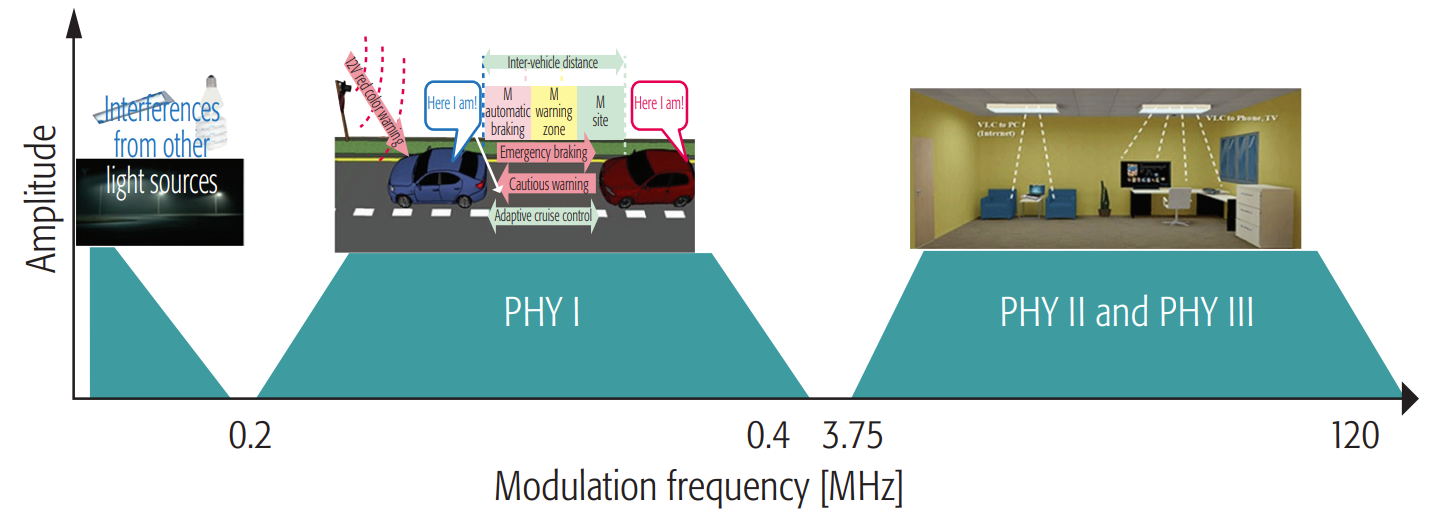
\includegraphics[scale=0.35]{./figuras/capasEstandar.png}
    \caption{\small{División en frecuencia para los tres tipos de capas PHY. Fuente [X].}}
    \label{capasPHY}%
\end{figure}

Además, el estándar especifica tres clases de dispositivos VLC cuyas características 
concretas se muestran en la tabla 1.1. En dicha tabla se puede comprobar como la fuente de 
luz necesaria para la emisión y recepción es débil para móvil, pero debe ser intensa para 
infraestructuras y vehículos. Además, las infraestructuras no incluyen movilidad física 
mientras que tanto móviles como vehículos sí. Una característica muy importante es el 
rango de alcance, este rango es corto para móvil y largo para vehículos mientras que 
para infraestructuras puede ser corto o largo. Por último, se especifica la tasa de datos
(número de bits por unidad de tiempo) que es alta para móvil, baja para los vehículos y 
alta o baja para las infraestructuras.

\begin{table}[ht]
    \centering
    \begin{tabular}{c|
    >{\columncolor[HTML]{CBCEFB}}c |
    >{\columncolor[HTML]{DAE8FC}}c |
    >{\columncolor[HTML]{CBCEFB}}c |}
    \cline{2-4}
                                                                            & \textbf{Infraestructura} & \textbf{Móvil} & \textbf{Vehículo} \\ \hline
    \multicolumn{1}{|c|}{\cellcolor[HTML]{DAE8FC}\textbf{Fuente de luz}}    & Intensa                  & Débil          & Intensa           \\ \hline
    \multicolumn{1}{|c|}{\cellcolor[HTML]{DAE8FC}\textbf{Movilidad física}} & No                       & Sí             & Sí                \\ \hline
    \multicolumn{1}{|c|}{\cellcolor[HTML]{DAE8FC}\textbf{Rango}}            & Corto/Largo              & Corto          & Largo             \\ \hline
    \multicolumn{1}{|c|}{\cellcolor[HTML]{DAE8FC}\textbf{Tasa de datos}}    & Alta/Baja                & Alta           & Baja              \\ \hline
    \end{tabular}
    \caption{\small{Clasificación de dispositivos según el estándar IEEE 802.15.7. Fuente [6]}}
\end{table}

Este estándar proporciona una visión global y común para las comunicaciones ópticas 
inalámbricas de corto alcance. Además, asegura inmunidad a interferencias 
electromagnéticas y a sistemas radiofrecuencia.

\section{Enlace de luz}
Para probar el proyecto y verificar el funcionamiento real del mismo
se parte de un enlace de luz formado por un transmisor y un 
receptor. A continuación, se van a describir brevemente para tener una idea de 
su funcionamiento e importancia ya que han sido 
heredados y no han sido desarrollados en este proyecto. Pero antes la figura 
\ref{enlace}
muestra el enlace completo durante una transmisión a pocos metros en el laboratorio.

\begin{figure}[ht]
    \centering
    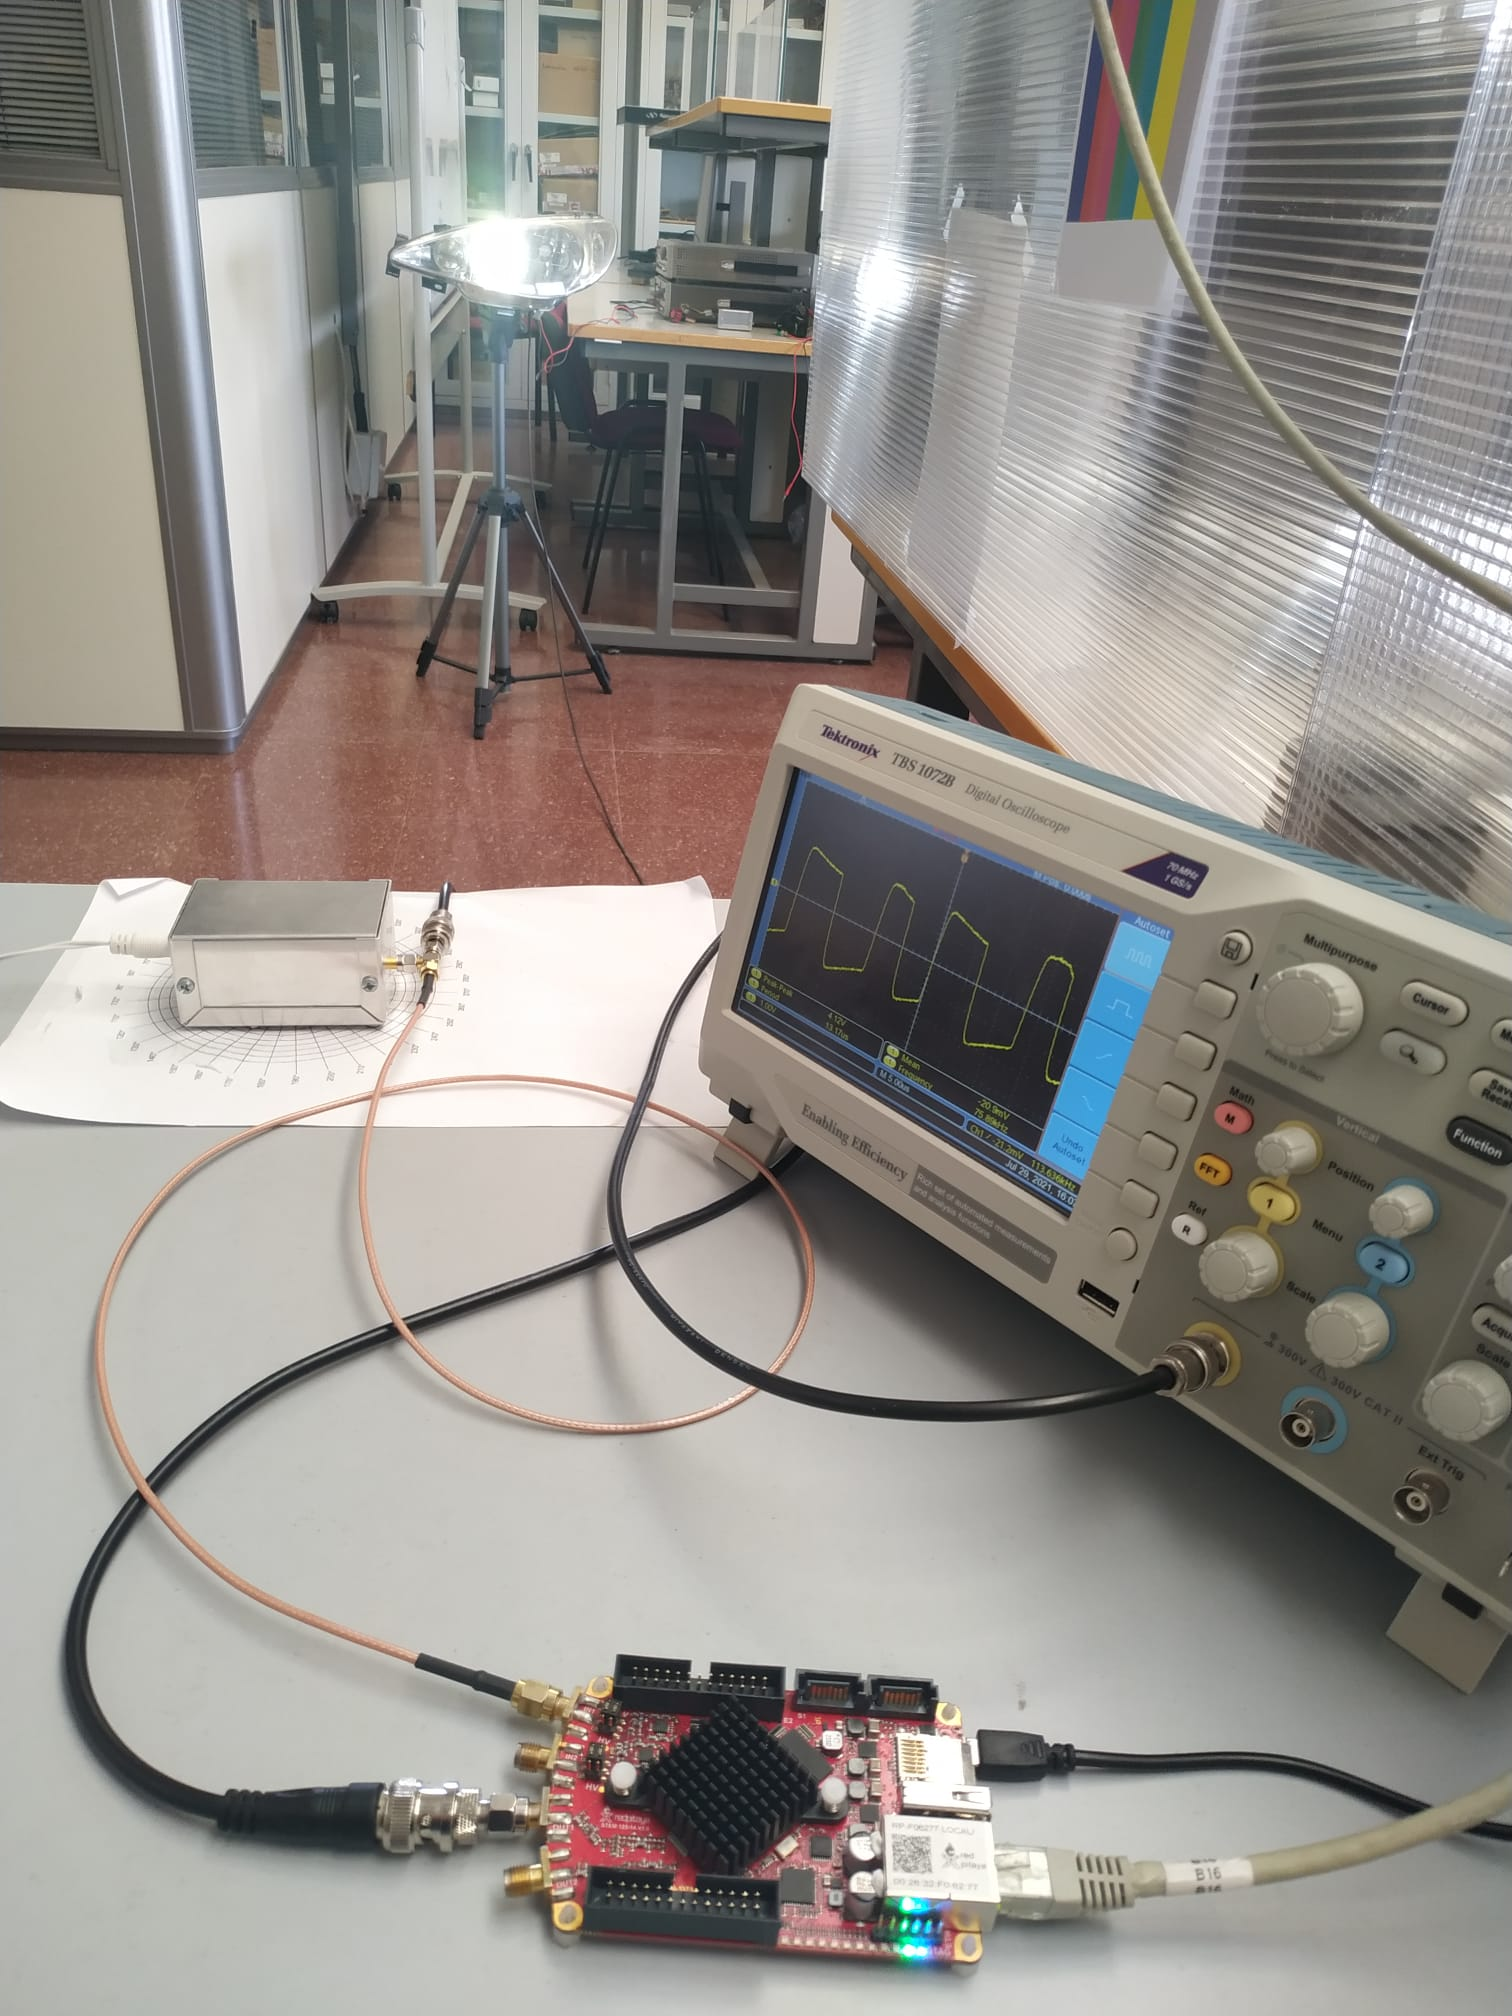
\includegraphics[scale=0.15]{./figuras/Enlace.jpeg}
    \caption{\small{Sistema de transmisión-recepción completo.}}
    \label{enlace}%
\end{figure}

\subsection{Transmisor}
%Hablar un poco del transmisor óptico que tiene Salva y de los voltajes.
El funcionamiento del transmisor se puede desglosar en tres etapas:
\begin{itemize}
    \item Adaptación de nivel: se encarga de convertir los niveles logicos de la señal 
    de entrada ('1' codificado como 1 V y '0' codificado como –1 V) en niveles de tensión 
    utiles para el modulador.
    \item Ajuste de corriente: su función es excitar a los dispositivos
    LED con la corriente reconfigurada.
    \item Habilitación de baja frecuencia: Por debajo de 100 KHz, el nivel de tension alto 
    que se entrega al modulador desciende abruptamente y el ciclo de trabajo de la senal se 
    ve dañado por lo que esta etapa consiste en eliminar dicha restricción.
\end{itemize}

Lo más importante del transmisor es conocer los niveles de amplitud para saber lo que 
tiene que proporcionarle la FPGA. En este caso la amplitud a nivel alto es de 1V y a nivel 
bajo es de 0V. 

En la figura x se muestra una imagen del transmisor óptico.

[FOTO DEL TRANSMISOR DE SALVA]

Este dispositivo ha sido incorporado a un faro de coche para que la simulación de la 
transmisión sea más realista como se ve en la figura x.

[FOTO DEL FARO]

\subsection{Receptor}
%Hablar un poco del receptor óptico que tiene Salva y de los voltajes.
El funcionamiento del receptor se puede desglosar en tres etapas:
\begin{itemize}
    \item Fotodetector: se encarga de transformar la luz pulsada emitida por el transmisor
    en corriente.
    \item Amplificador de transimpedancia: realiza la tarea de convertir la corriente del 
    fotodetector en tensión.
    \item Amplificador no inversor: amplifica la señal para dar más sensibilidad al 
    receptor.
\end{itemize}

Como se comentó en el transmisor lo importante son los niveles de amplitud que, en este 
caso, son de 1V a nivel alto y de -1V a nivel bajo. Este rango es el que tiene la 
FPGA a la entrada por lo que nos proporciona una resolución máxima.

En la figura x se muestra una imagen del receptor óptico.

[FOTO DEL RECEPTOR DE SALVA]

\section{Sistema de partida}
% Hablar sobre el proyecto que nos dejó Andrés tanto de las características
% software como su capacidad de alcance y el enfoque del trabajo de Andrés que era el Desarrollo
% del filtro adaptado y al final tratar de hilarlo con nuestra implementación para mejorar el sistema.
% Comentar el mapeo de la señal para ponerla en el rango [-8192,8191] que nos influye para el hard-decoding y el soft-decoding.
Hay que mencionar que este trabajo coge el testigo de otro trabajo desarrollado con
anterioridad. Dicho trabajo consiste, a grandes rasgos, en el desarrollo del filtro 
adaptado para mejorar la comunción por luz visible. 

El funcionamiento del sistema, de manera general, se divide en dos bloques. Transmisión y 
recepción. 

La transmisión consiste en que un programa en C 
produce una trama que se almacena en la memoria RAM y se pasa a los bloques encargados
de su transmisión como son el serializador, el modulador y finalmente el DAC para 
transformar el dato digital en analógico y el transmisor óptico para transmitir la señal
en forma de pulsos de luz. 

La señal se recibe por el receptor óptico y este la pasa el conversor ADC para volver 
a digitalizar la señal para que pueda ser procesada. Es en este momento, donde actúa el 
filtro adaptado. Su función principal, de una manera resumida, consiste en detectar la 
presencia de una señal conocida o patrón dentro de la señal recibida. La señal a la
salida será la correlación entre la conocida y la recibida. Esto es correspondiente
a realizar la convolución de la señal desconocida con una que usa como referencia.
Por tanto, el objetivo del filtro adaptado es el de maximizar la relación señal a rudi 
(SNR) de una señal conocida para poder recuperarla por completo.

Después de  ser filtrada por el filtro adaptado, la señal se demodula y los datos se 
guardan
en la memoria RAM para que puedan ser leídos el programa en C anteriormente mencionado.

En el siguiente apartado, se van a describir las mejoras que se han decidido
implementar para mejorar sus prestaciones y acercar más el funcionamiento del sistema 
a lo requerido para poder ser implementado en aplicaciones vehículares en las que las 
distancias de transmisión son más largas ya que el sistema anterior no permitía 
transmisiones de larga distancia. 

\section{Mejoras respecto al sistema anterior}
% Hablar sobre cuales son las mejoras que se han implementado y que es lo que se quiere conseguir con estas mejoras.
% Las mejoras (Mayor robustez de paquetes y mayor distancia de transmisión) se han conseguido
% gracias a implementar esquemas de codificación y sistemas de decisión.
Tras analizar el proyecto del que se partía se concluyó que había que desarrollar algún 
subsistema para mejorar el enlace y acercarlo a que pueda ser utilizado en aplicaciones
vehículares de manera eficaz. Una manera de mejorar el 
sistema de comunicación y seguir el camino de investigar los sistemas de comunicación por 
luz visible era desarrollar e implementar varios esquemas de señalización y varios sistemas
de decisión de la señal para analizar sus diferentes comportamientos y cuantificar las 
mejoras. Estas mejoras, principalmente, están centradas en proporcionar mayor robustez al 
sistema para poder interpretar y decodificar la señal de la mejor manera posible cuando
se trabaje en condiciones adversas como pueden ser situaciones en las que la señal se 
mezcle con mucho ruido o simplemente cuando se transmita información a mucha distancia y 
la fuerza de la señal disminuya.

En los siguientes apartados se van a desarrollar tanto su fundamento teórico como su 
implementación en una FPGA tanto de los esquemas de señalización como de los 
sistemas de decisión. Además de realizar las respectivas pruebas para verificar las
mejoras que se producen.

\chapterend{}


% Capítulo 04.
%%%%%%%%%%%%%%%%%%%%%%%%%%%%%%%%%%%%%%%%%%%%%%%%%%%%%%%%%%%%%%%%%%%
%%% Documento LaTeX 																						%%%
%%%%%%%%%%%%%%%%%%%%%%%%%%%%%%%%%%%%%%%%%%%%%%%%%%%%%%%%%%%%%%%%%%%
% Título:		Capítulo 3
% Autor:  	Ignacio Moreno Doblas
% Fecha:  	2014-02-01, actualizado 2019-11-11
% Versión:	0.5.0
%%%%%%%%%%%%%%%%%%%%%%%%%%%%%%%%%%%%%%%%%%%%%%%%%%%%%%%%%%%%%%%%%%%
% !TEX root = A0.MiTFG.tex

\chapterbegin{Fundamentos teóricos}
\label{chp:App}
\minitoc

\section{Introducción a los esquemas de señalización}
%Hablar sobre qué són los esquemas de señalización y cual es su función principal. comentar
%los esquemas (alternos,cancelación,4ppm,4ippm y pwm) y por qué se han elegido o descartado.
%Decir que no son los esquemas del estándar y que se han elegido para investigar sus ventajas e inconvenientes. 

En el ámbito de la comunicación existen múltiples esquemas de codificación digital con diferentes propiedades como 
probabilidad de bit, ciclo de trabajo, ancho de banda, etc. A la hora de estudiar un esquema de codificación para hacer 
su elección hay que tener en cuenta tres aspectos fundamentales, que son:
\begin{itemize}
    \item Flickering: se define como el cambio de la luz provocado por la conmutación entre encendido 
y apagado (1 y 0) en intervalos muy cortos. 
Estos parpadeos, si se producen a una velocidad perceptible por el ojo humano, pueden llegar a ser molestos y causar dolor. 
    \item Rendimiento óptico.
    \item La capacidad para controlar la atenuación o el dimming, provocado por por la variación de la intensidad de la luz, 
    en esquemas de codificación con ancho de pulso de la señal variable. 
\end{itemize} 

El estándar de comunicaciones por luz visible IEEE 802.15.7 usa como esquema de señalización la codificación Manchester. 
Continuando con el estudio de los esquemas de señalización,
a continuación, se van a desarrollar otras opciones de esquemas de codificación con características diferentes
para estudiar su eficacia e impacto en las comunicaciones por luz visible.
Los esquemas a desarrollar son codificación por pulsos alternos, cancelación de pulsos y 4-ppm. También se hará una 
comparativa de 4-ppm frente a Inverse 4-ppm para comparar sus prestaciones y el efecto de transmitir mayor cantidad 
de ``unos'' que de ``ceros''.

Es importante destacar que en un primer momento también se planteó el desarrollo de codificación 4-PWM pero se descartó su 
implementación debido a su escasa capacidad para controlar el dimming. Esto provocaba que la intensidad de la luz 
fluctuara mucho a lo largo de una transmisión siendo perceptible y molesto para el ojo humano.

\section{Pulsos alternos}
Comentar teóricamente en que consiste este esquema (miller pero con una opción menos y alternando).
Y que apenas está implementado y desarrollado en ningún sitio.

Dibujar y comentar el diagrama de trellis de este esquema para la codificación/decodificación de la señal.
\vspace{2cm}

\begin{figure}[ht]
    \centering
    %   TRELLIS PULSOS ALTERNOS

\tikzstyle{state}=[shape=circle,draw=blue!50,fill=blue!20,inner sep=2pt]
\def\desp{1.5}%
\begin{tikzpicture}[]
% 1st column
\draw (0,\desp) node[name=s1_1,state] {$S_1$} node[xshift=-2.2cm]{$0/00$}node[xshift=-1cm]{$1/01$};
\draw (0,0) node[name=s2_1,state] {$S_2$} node[xshift=-2.2cm]{$0/00$}node[xshift=-1cm]{$1/10$};
% 2nd column

\node[state] (s1_2) at (2,\desp) {$S_1$}
    edge[dashed] (s1_1)
    edge[thin] (s2_1);
\node[state] (s2_2) at (2,0) {$S_2$}
    edge[thin] (s1_1)
    edge[dashed] (s2_1);

% 3rd column

\node[state] (s1_3) at (4,\desp) {$S_1$}
    edge[dashed] (s1_2)
    edge[thin] (s2_2);
\node[state] (s2_3) at (4,0) {$S_2$}
    edge[thin] (s1_2)
    edge[dashed] (s2_2);
\end{tikzpicture}

\hspace{1cm}--------- $1$ ---------

\hspace{1cm} - - - - - $0$ - - - - -

    \caption{\small{Diagrama de Trellis de la codificación pulsos alternos.}}
    \label{trellis_alternos}%
\end{figure}

si encuentro algo hablar sobre cual es su espectro y las diferencias respecto a los del estándar

Desarrollar por qué es un esquema no equiprobable haciendo los cálculos correspondientes.

Comentar si se encuentra la ber y sus prestaciones

\section{Pulsos alternos con cancelación de pulsos}
Comentar teóricamente en que consiste este esquema (alternos pero eliminando pulsos).
Y que apenas está implementado y desarrollado en ningún sitio.

Dibujar y comentar el diagrama de trellis de este esquema para la codificación/decodificación de la señal.

\begin{figure}[ht]
    \centering
    %CANCELACION
\tikzstyle{state}=[shape=circle,draw=blue!50,fill=blue!20,inner sep=2pt]
\def\desp{1.5}%
\begin{tikzpicture}[]
% 1st column
\draw (0,3*\desp) node[name=s1_1,state] {$S_1$} node[xshift=-2.2cm]{$0/00$}node[xshift=-1cm]{$1/00$};
\draw (0,2*\desp) node[name=s2_1,state] {$S_2$} node[xshift=-2.2cm]{$0/10$}node[xshift=-1cm]{$1/01$};
\draw (0,\desp) node[name=s3_1,state] {$S_3$} node[xshift=-2.2cm]{$0/00$}node[xshift=-1cm]{$1/00$};

% 2nd column

\node[state] (s1_2) at (2,3*\desp) {$S_1$}
    edge[dashed] (s1_1)
    edge[dashed] (s2_1)
    edge[dashed] (s3_1);
\node[state] (s2_2) at (2,2*\desp) {$S_2$}
    edge[thin] (s1_1)
    edge[thin] (s3_1);
\node[state] (s3_2) at (2,\desp) {$S_3$}
    edge[thin] (s2_1);

% 3d column

\node[state] (s1_3) at (4,3*\desp) {$S_1$}
    edge[dashed] (s1_2)
    edge[dashed] (s2_2)
    edge[dashed] (s3_2);
\node[state] (s2_3) at (4,2*\desp) {$S_2$}
    edge[thin] (s1_2)
    edge[thin] (s3_2);
\node[state] (s3_3) at (4,\desp) {$S_3$}
    edge[thin] (s2_2);


\end{tikzpicture}

\hspace{1cm}--------- $1$ ---------

\hspace{1cm}- - - - - $0$ - - - - -
%\line(1,0){2cm}  $1$ \line(1,0){2cm}


% 1 linea continua, 0 linea discontinua
    \caption{\small{Diagrama de Trellis de la codificación cancelación de pulsos.}}
    \label{trellis_cancelacion}%
\end{figure}

si encuentro algo hablar sobre cual es su espectro y las diferencias respecto a los del estándar

Desarrollar por qué es un esquema no equiprobable haciendo los cálculos correspondientes.

Comentar si se encuentra la ber y sus prestaciones

\section{4-PPM}
Explayarme mucho más porque hay mucha más información.
Comentar teóricamente en que consiste este esquema.
Y que apenas está implementado y desarrollado en ningún sitio.

Dibujar y comentar el diagrama de trellis de este esquema para la codificación/decodificación de la señal.

si encuentro algo hablar sobre cual es su espectro y las diferencias respecto a los del estándar

Desarrollar por qué es un esquema no equiprobable haciendo los cálculos correspondientes.

Comentar si se encuentra la ber y sus prestaciones

\section{Comparativa 4-PPM frente a Inverse 4-PPM}
Comparar estos dos esquemas y comentar ventajas e inconvenientes.
%https://ieeexplore.ieee.org/stamp/stamp.jsp?tp=&arnumber=6614862
%https://ieeexplore.ieee.org/stamp/stamp.jsp?tp=&arnumber=567560&tag=1

\section{Sistemas de decisión}
%Hablar sobre las técnicas usadas --> hard-decoding, soft-decoding y algoritmo de Viterbi
%Tener en cuenta el mapeo que se realiza para poner la señal en el rango [-8192,8191]
En este apartado se van a describir los diferentes sistemas de decisión para interpretar la señal recibida de la mejor 
manera posible que se han implementado. Para ello, se van a desarrollar 
sus características más representativas así como sus ventajas e inconvenientes.

\subsection{Hard-decoding}


\subsection{Soft-decoding}
aaaaaaaaaa
aaaaaaaaaa

aaaaaaaa
\subsection{Algoritmo de Viterbi}

% \begin{figure}[htbp]
%     \centering
%     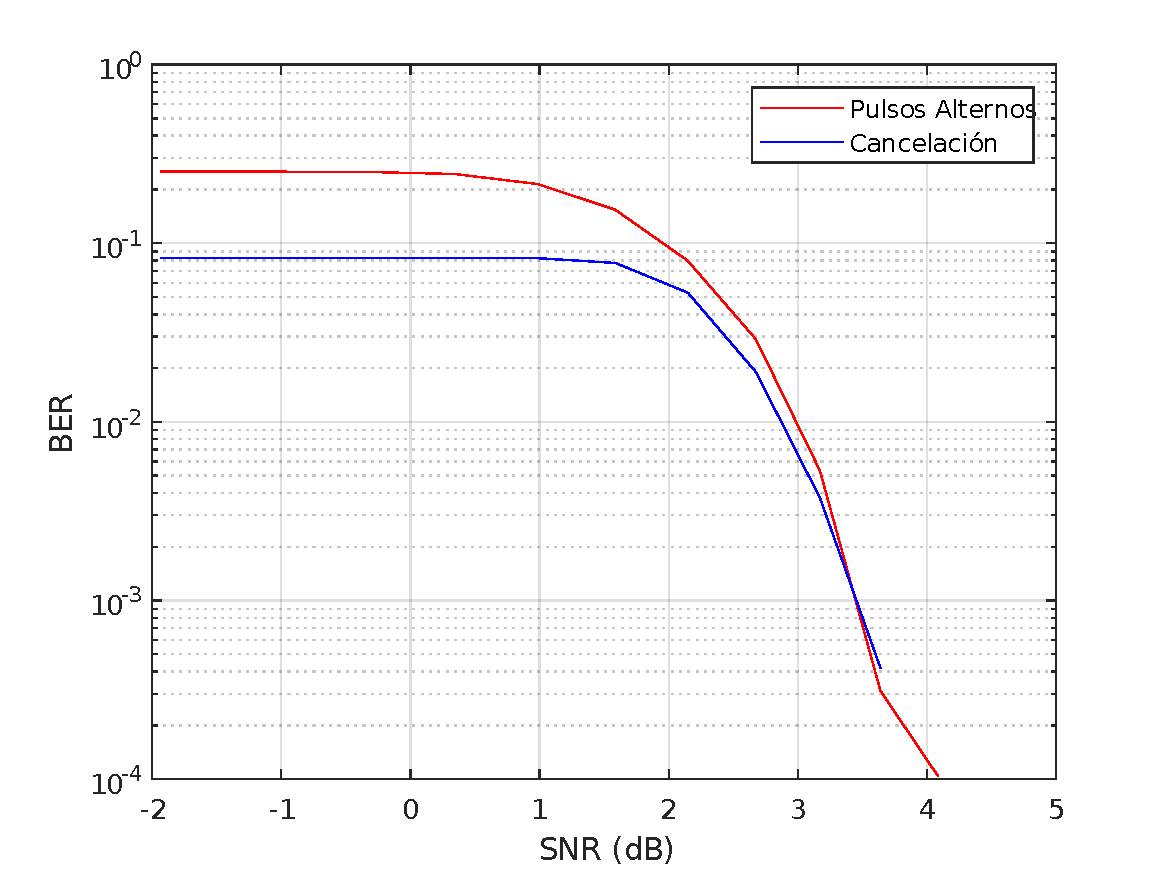
\includegraphics[scale=0.75]{./figuras/Viterbi_pulsos_cancelacion.pdf}
%     \caption{\small{Viterbi.}}
%     \label{Viterbi}%
% \end{figure}

\subsection{Comparativa entre los sistemas de decisión}
A continuación, se va a comparar la tasa de error de bit (BER) de los distintos esquemas de decisión, para cada esquema 
de codificación, en función de la relación señal a ruido (SNR), que varia con la distancia (disminuyendo la 
amplitud de la señal), para verificar la mejora que se produce entre cada sistema de decisión.

Para pulsos alternos, la principal mejora se nota con la aplicación del algoritmo de Viterbi.

Para cancelación de pulsos la aplicación del algoritmo de Viterbi es muy importante ya que, como se comentó anteriormente,
se descartan muchas opciones al mirar un pasado.

Para 4ppm el uso de soft-decoding implica una gran mejora debido a la posibilidad de buscar el bit mayor ya que solo 
se recibe un '1' por cuarteto de bits.

%%FOTOS DE ALTERNOS (HARD,SOFT,VITERBI), CANCELACION (HARD,SOFT,VITERBI) Y 4PPM(HARD,SOFT)

%%%%%%%% NO SE SI PONER UN APARTADO DE COMPARATIVA ENTRE CODIFICACIONES SEGUN EL SISTEMA DE DECISION O PONER LAS FOTOS
%%% DENTRO DE CADA ESQUEMA %%%%%%%%%%%%%%%%%%%%%%%%%%


\chapterend{}


% Capítulo 05.
%%%%%%%%%%%%%%%%%%%%%%%%%%%%%%%%%%%%%%%%%%%%%%%%%%%%%%%%%%%%%%%%%%%
%%% Documento LaTeX 																						%%%
%%%%%%%%%%%%%%%%%%%%%%%%%%%%%%%%%%%%%%%%%%%%%%%%%%%%%%%%%%%%%%%%%%%
% Título:		Capítulo 5
% Autor:  	Ignacio Moreno Doblas
% Fecha:  	2014-02-01, actualizado 2019-11-11
% Versión:	0.5.0
%%%%%%%%%%%%%%%%%%%%%%%%%%%%%%%%%%%%%%%%%%%%%%%%%%%%%%%%%%%%%%%%%%%
% !TEX root = A0.MiTFG.tex

\chapterbegin{Implementación}
\label{chp:App2}
\minitoc

\section{Sistema general}
Comentar como se relacionan los bloques entre sí y el orden de los mismos para luego entrar en profundidad en 
los bloques que se han desarrollado.

\section{Transmisor}
		-Selector del esquema de codificación (sincronismo manchester y trama en la codificación elegida)
		-Diagramas de Markov para implementar la codificación

\section{Receptor}
		-Recepción del dato serie
		-Agrupar los datos en parejas o cuartetos
		-Decodificar con máquinas de estados o identificación del bit mayor.

\section{Sistema de decisión} (hard-soft decoding, algoritmo de viterbi)
		-Hard-decoding (umbral en la mitad)
		-Soft-decoding (cómo se implementa el cálculo de la distancia euclídea)
		-Algoritmo de Viterbi (que efecto tiene y cómo se implementa la mirada al pasado para descartar opciones que tienen probabilidad 0)
\chapterend{}

% Capítulo 06
%%%%%%%%%%%%%%%%%%%%%%%%%%%%%%%%%%%%%%%%%%%%%%%%%%%%%%%%%%%%%%%%%%%
%%% Documento LaTeX 																						%%%
%%%%%%%%%%%%%%%%%%%%%%%%%%%%%%%%%%%%%%%%%%%%%%%%%%%%%%%%%%%%%%%%%%%
% Título:		Capítulo 5
% Autor:  	Ignacio Moreno Doblas
% Fecha:  	2014-02-01, actualizado 2019-11-11
% Versión:	0.5.0
%%%%%%%%%%%%%%%%%%%%%%%%%%%%%%%%%%%%%%%%%%%%%%%%%%%%%%%%%%%%%%%%%%%
% !TEX root = A0.MiTFG.tex

\chapterbegin{Pruebas}
\label{chp:App3}
\minitoc

\chapterend{}


\part{Parte tercera.}
% !TEX root = A0.MiTFG.tex

\chapterbeginx{Conclusiones y líneas futuras}

Después de todo el desarrollo del proyecto, es pertinente hacer una
valoración final del mismo, respecto a los resultados obtenidos, las
expectativas o el resultado de la experiencia acumulada.

Esta sección es indispensable y en ella se ha de reflejar, lo más
claramente posible, las aportaciones del trabajo con unas conclusiones
finales.

Además, considerando también el estado de la técnica, se deben indicar
las posibles líneas futuras de trabajo, proponer otros puntos de vista
o cualquier otra sugerencia como postámbulo del presente trabajo, para
ser considerada por el lector o el tribunal evaluador.


\chapterend


% Anexos
\part{Apéndices}

\appendix

%%%%%%%%%%%%%%%%%%%%%%%%%%%%%%%%%%%%%%%%%%%%%%%%%%%%%%%%%%%%%%%%%%%
%%% Documento LaTeX 																						%%%
%%%%%%%%%%%%%%%%%%%%%%%%%%%%%%%%%%%%%%%%%%%%%%%%%%%%%%%%%%%%%%%%%%%
% Título:		Apéndice A
% Autor:  	Ignacio Moreno Doblas
% Fecha:  	2014-02-01, actualizado 2019-11-11
% Versión:	0.5.0
%%%%%%%%%%%%%%%%%%%%%%%%%%%%%%%%%%%%%%%%%%%%%%%%%%%%%%%%%%%%%%%%%%%%

\pagestyle{fancy}
\fancyhead[LE,RO]{\thepage}
\fancyhead[RE]{Apéndice} %
\fancyhead[LO]{\nouppercase{\rightmark}}

\chapter{Manual de uso}

\minitoc

\section{Primera sección}


\chapterend


%\input{D2.AppendixB.tex}

%\input{D3.AppendixC.tex}

% Formato de documento en la parte final.
\backmatter
%Hace que los capítulos y títulos nivel inferior no aparezcan numerados (lo que es ideal para conclusiones o notas finales).

% Bibliografía
%%%%%%%%%%%%%%%%%%%%%%%%%%%%%%%%%%%%%%%%%%%%%%%%%%%%%%%%%%%%%%%%%%%
%%% Documento LaTeX 																						%%%
%%%%%%%%%%%%%%%%%%%%%%%%%%%%%%%%%%%%%%%%%%%%%%%%%%%%%%%%%%%%%%%%%%%
% Título:		Bibliografía
% Autor:  	Ignacio Moreno Doblas
% Fecha:  	2014-02-01, actualizado 2019-11-11
% Versión:	0.5.0
%%%%%%%%%%%%%%%%%%%%%%%%%%%%%%%%%%%%%%%%%%%%%%%%%%%%%%%%%%%%%%%%%%%%

% Encabezamiento %
\pagestyle{fancy}
\fancyhead[LE,RO]{\thepage}
\fancyhead[RE,LO]{Bibliografía}

%Inclusión de bibliografía%
\bibliography{E2.Bibliografia} %Úsese el nombre del fichero sin extensión

%Inclusión en el índice (Tabla de contenidos)
\addcontentsline{toc}{chapter}{Bibliografía}

%Formateo de estilo de bibliografía
% Otros formatos: plain, unsrt, abbrv
%  plain: las entradas se ordenan alfabéticamente y se etiquetan con un número (p.ej., [1])
% unsrt: igual que plain, pero aparecen en orden de citación.
% alpha: el etiquetado se hace por autor y año de publicación (p.ej., [Knu66]).
% abbrv: igual que alpha, pero más abreviado.
\bibliographystyle{unsrt}

%Impresión de todas las entradas bibliográficas aunque no estén citadas
%\nocite{*}

\chapterend


% Índice alfabético%
%%%%%%%%%%%%%%%%%%%%%%%%%%%%%%%%%%%%%%%%%%%%%%%%%%%%%%%%%%%%%%%%%%%
%%% Documento LaTeX 																						%%%
%%%%%%%%%%%%%%%%%%%%%%%%%%%%%%%%%%%%%%%%%%%%%%%%%%%%%%%%%%%%%%%%%%%
% Título:		Glosario (index)
% Autor:  	Ignacio Moreno Doblas
% Fecha:  	2014-02-01, actualizado 2019-11-11
% Versión:	0.5.0
%%%%%%%%%%%%%%%%%%%%%%%%%%%%%%%%%%%%%%%%%%%%%%%%%%%%%%%%%%%%%%%%%%%%

\pagestyle{fancy}
\fancyhead[LE,RO]{\thepage}
\fancyhead[RE,LO]{Glosario} 

\printindex

%Example 	Index Entry 	Comment
%\index{hello} 	hello, 1 	Plain entry
%\index{hello!Peter} 	  Peter, 3 	Subentry under 'hello'
%\index{Sam@\textsl{Sam}} 	Sam, 2 	Formatted entry
%\index{Lin@\textbf{Lin}} 	Lin, 7 	Same as above
%\index{Jenny|textbf} 	Jenny, 3 	Formatted page number
%\index{Joe|textit} 	Joe, 5 	Same as above
%\index{ecole@\'ecole} 	école, 4 	Handling of accents
%\index{Peter|see{hello}} 	Peter, see hello 	Cross-references
%\index{Jen|seealso{Jenny}} 	Jen, see also Jenny 	Same as above


\chapterend


\end{document}
